\documentclass{article}

\usepackage[latin1]{inputenc}
\usepackage[T1]{fontenc}
\usepackage{amsmath}
\usepackage{multicol}
\usepackage{graphics}



\begin{document}
\parbox{3cm}{ 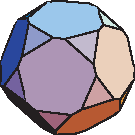
\includegraphics{images/fig4}} \parbox{11.5cm}{ En
	{\sc Mathematica}, podemos eliminar una o varias caras de un dodecaedro,
	seleccionar el color y el grosor de las aristas y poner color a las caras.
	Para esto debemos utilizar los comandos ... }

\end{document}